\section{Experiment Setup}
The quantitative comparison is done by help of several experiments on the two versions of the CoAP protocol. For these experiments different setups are made, all based on the IoTivity framework running on two Linux (Ubuntu) machines. These two machines are both wireless coupled to a local network via a router. The test case for the experiments is meant to represent a constrained device, acting as a client, updating the temperature on a cloud server with a specific interval of time. 

Linux is chosen to represent a constrained device as it is necessary to be able to easily monitor the communication from the client side of view.

The setup for CoAP over UDP as illustrated in \figurename \ref{fig:setup}, uses two applications. A simple IoTivity client and server application both developed in C++ using CoAP over UDP as an application protocol.
\begin{figure}[bht]
	\centering
	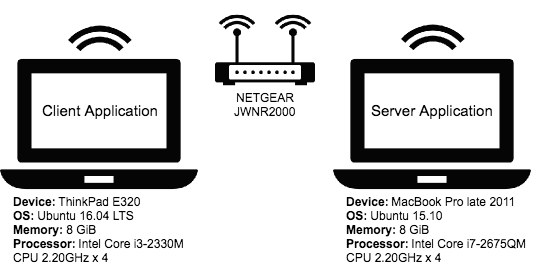
\includegraphics[width=3in]{gfx/setupa}
	\caption{Setup for CoAP over UDP.}
	\label{fig:setup}
\end{figure}

Setup for CoAP over TCP as illustrated in \figurename \ref{fig:setup} uses two applications. A simple IoTivity client application developed in C++ and a simple IoTivity server application developed in Java. Both applications uses CoAP over TCP as an application protocol.

%Wireshark....
%\textbf{Memory consumption}\\
%Flyt den del til et afsnit med prototype implementation (før resultaterne)
%How much memory usage...
